%Autor: Simon Walker
%Version: 1.0
%Datum: 25.06.2020
%Lizenz: CC BY-NC-SA


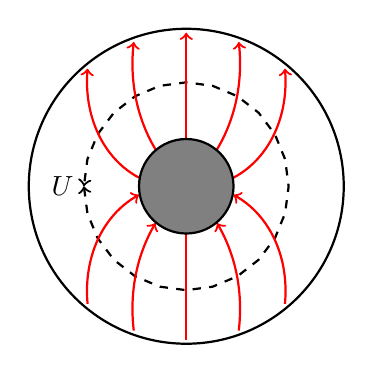
\begin{tikzpicture}

%Mittlerer Umfang
\draw[<->, 
dashed, 
thick, 
domain=180:540, 
variable=\x] 
plot ({1.3*cos(\x)}, {1.32*sin(\x)})
node[left] {$U$};


%Feldlinien
\draw[red, thick, ->] (0, 0.6) -- (0, 1.95);
\draw[red, thick, ->, domain=0.61:1.95, variable=\x] plot ({130-20/(1.35/(\x-0.6))}:\x);
\draw[red, thick, ->, domain=0.61:1.95, variable=\x] plot ({50+20/(1.35/(\x-0.6))}:\x);
\draw[red, thick, ->, domain=0.61:1.95, variable=\x] plot ({170-40/(1.35/(\x-0.6))}:\x);
\draw[red, thick, ->, domain=0.61:1.95, variable=\x] plot ({10+40/(1.35/(\x-0.6))}:\x);

\draw[red, thick, <-] (0, 0.6) -- (0, -1.95);
\draw[red, thick, <-, domain=0.61:1.95, variable=\x] plot ({-130+20/(1.35/(\x-0.6))}:\x);
\draw[red, thick, <-, domain=0.61:1.95, variable=\x] plot ({-50-20/(1.35/(\x-0.6))}:\x);
\draw[red, thick, <-, domain=0.61:1.95, variable=\x] plot ({-170+40/(1.35/(\x-0.6))}:\x);
\draw[red, thick, <-, domain=0.61:1.95, variable=\x] plot ({-10-40/(1.35/(\x-0.6))}:\x);


\draw[thick] (0,0) circle (2); %Ausserer Kreis
\draw[thick, fill=gray] circle (0.6); %Innerer Kreis
\end{tikzpicture}
